El orden en que escribí el código fue primero el FS, luego el kernel y por
último las utilidades. Sin embargo para hacerlo más consistente se presentará
primero el kernel, que pega todos los componentes y facilita la explicación del
FS y las utilidades.

El kernel está basado en el utilizado en la cursada de Organización del
Computador 2, 2do cuatrimestre del 2010. En este sistema armamos las
estructuras necesarias para bootear un sistema en modo protegido con paginación.
Esto incluye un bootloader que carge la imagen, el manejo del A20, y llenado de
GDT/IDT/TSS etc. Esto permitía manejo de interrupciones y dio lugar a un simple
scheduler que daba una forma primitiva de multiprogramación.

Si bien partí de esta base de código, muchos de los componentes fueron
modificados o reescritos totalmente. Los cambios más importantes fueron en el
scheduler (conjunto con el manjeo de tss), el manejo de procesos, el mmu o
manejo de la memoria y el manejo del teclado/pantalla.

Ya teniendo un núcleo booteable con el que trabajar me hizo pensar que los
cambios no iban a requerir demasiado trabajo. Estaba seriamente equivocado. Si
bien grandes partes del código las implementaba rápido y bien en general en la
primera pasada, eran los pequeños errores, un bit incorrecto en el lugar menos
esperado, que me robaba horas (o hasta días algunos casos) intentando de
arreglar. Esto me hizo recordar la ley de Hofstadter: "It always takes longer
than you expect, even when you take into account Hofstadter's Law"

Antes de comenzar a hablar sobre cada componente en detalle, voy a dar algunas
características generales del kernel. Este núcleo utiliza la idea de "Lower
Half Kernel", o kernel en la parte baja de la memoria. Esto significa que la
imagen del kernel se copia y mapea virtualmente en los primeros 4mb de la
memoria. En un principio pensé utilizar la idea de "Higher Half Kernel" en
donde el mapeo se hace al final de la memoria (en general al rededor de los
3gb), que es la que se utiliza en las kernels modernas (linux, windows, bsd,
etc), haciendo la carga de los programas más simple y por sobretodo
manteniendome en el standar. Sin embargo debido a no tener control sobre el
bootloader, y no siendo este compatible con multiboot, me fue imposible
controlar la carga de la imagen y por ende abandoné la idea.

Las implicaciónes de esta decisión fueron que al compilar las aplicaciónes de
usuario, estas deben empezar con el offset de 4mb, o 0x400000 en hexa, para que
tengan sentido todos los punteros. Para ver más sobre esta explicación,
dirigirse a la sección "Manejo de Procesos" y "Utilidades" al final del
informe.

Desde un primer momento me propuse implementar una interfaz con el usuario del
tipo POSIX, es decir utilizar al igual que linux/bsd la interrupción 0x80 para
manejar llamadas al sistema. Respeté todos las signaturas de las llamadas POSIX
(exit/open/close/write/etc.), sus números de interrupción, logrando de esta
manera tener un sistema "compatible" con linux. Si bien obviamente esta
compatibilidad es muy reducida, en la sección de utilidades se mostrará como
todas las aplicaciónes programadas para esta kernel funcionan sin ninguna
modificación en un sistema linux.

Otro punto importante es el uso de sys/queue.h. Este header extraido de minix
(que a su vez fue extraido de NetBSD) contienen una implementación estándar
varios tipos de listas (comunes, doble enlazadas, circulares, etc). Esto es
utilizado en varias partes, incluyendo el scheduler, el manejo de memoria, y en
el fs. Para entender más sobre esto dirigirse a sus respectivas páginas en el
manual ("man queue").

\subsection{Biblioteca General}

Al codificar los distintos componentes del núcleo, me di cuenta rápidamente que
existía un set de funciones básicas que eran útiles en muchas parte del código.
En su gran mayoría estas funciones eran imitaciones de aquellas en la
biblioteca estándar de C.

Es por esto que agregé al build la carpeta lib/, que contiene los archivos
lib/misc.c y lib/misc.h. Aquí implementé algunas de las funciones de libc que
necesitaba en más de un lugar, y eran lo suficientemente genéricas como para
que se puedan reutilizar. Decidí mantenerles el nombre que tienen en libc,
agregandole el prefijo "my". Si bien esto no corresponde extrictamente a la
explicación del kernel, me pareció correcto nombrarlas en este momento ya que
se verán a través de todo el código del kernel/fs/utilidades.

Así es como nacieron mystrlen(), mystrncmp(), mystrncpy(), mymemcpy(),
mymemset(), MIN() y space(). Todas estas funciones se comportan de la manera
que uno espera que funcionen, son compatibles con sus clones.

\subsection{Manejo de Procesos}

El manejo de procesos en el kernel se encarga de mantener información sobre
todos los procesos actualmente en el sistema, información relevante para el
scheduler/tty/fs etc. La implementación del mismo se encuentra en los archivos
kernel/sched.c y kernel/sched.h. Es importante notar que en el código, no hay
distinción entre manejo de procesos y scheduler, ambos se encuentran en el
mismo archivo.

Cada proceso en el sistema ocupa una pocisión en el arreglo "ps", de tipo
"struct process\_state\_s" definido en include/minikernel/sched.h. Esta
estructura contiene información como el pid/uid/gid del proceso, un puntero al
padre, la información del fs (directorio actual, descriptores de archivo
abiertos, etc), una serie de entradas de manejo de listas, y una lista de
páginas utilizadas. Toda esta información, más el estado del proceso guardado
en su respectivo TSS, define el estado de cualquier proceso en el sistema:

\begin{verbatim}
struct process_state_s {
    /* number */
    int i;

    /* process id */
    pid_t pid;

    /* parent */
    struct process_state_s *parent;

    /* process owner's uid and gid */
    pid_t uid;
    pid_t gid;

    /* data to keep track of waitpid sys call */
    struct process_state_s *waiting;
    int *status;
    pid_t child_pid;

    /* fs data */
    struct unused_fd_t unused_fd;
    struct file_s files[MAX_FILES];
    unsigned int curr_dir;

    /* dev io data */
    unsigned int dev;

    /* scheduler ready list pointers */
    CIRCLEQ_ENTRY(process_state_s) ready;

    /* scheduler waiting list pointers */
    LIST_ENTRY(process_state_s) wait;

    /* unused list pointers */
    LIST_ENTRY(process_state_s) unused;

    /* list of used pages */
    LIST_HEAD(pages_list_t, page_s) pages_list;
} __attribute__((__packed__)) ;
\end{verbatim}

En este archivo son definidas los handlers de todas las llamadas al sistema
que manejan procesos. Estas incluyen exit()/waitpid()/getpid() entre otras.

La llamada exit() se encarga de liberar todas las páginas pedidas por el
proceso, removerlo de la lista de procesos listos del scheduler, despertar al
padre si este estaba dormido esperandolo (con waitpid()), y programar el
siguiente proceso a ser ejecutado.

waitpid() recibe un pid de un proceso hijo, y bloquea al proceso que ejecuto la
llamada hasta que no termine el proceso hijo. Es utilizado por ejemplo en la
consola para esperar a que un comando enviado termine de ejecutarse. Logra esto
removiendo al proceso de la lista del scheduler, y apuntando en su estructura
al proceso que espera que termine. Lo despierta exit(). La forma de encontrar
al procesos hijo por su pid es mediante la función find\_pid(), que recorre la
lista de procesos buscando el deseado (recordando a Ken Thompson, uno de los
padres de Unix, When in doubt...).

getpid() simplemente devuelve el pid de la estructura "ps".

Obvié intencionalmente a las dos llamadas más importantes, fork() y execve().
En un principio comencé a utilizar este modelo para crear nuevos procesos, pero
resultó tener varias complicaciónes que no esperaba (en especial cuando se
realiza el fork() y no se sigue con el execv(), copiar el estado de un proceso
no era tan simple), por lo que decidí unir ambas llamadas y crear una nueva,
denominada newprocess(). Esta recibe los mismos parametros que execv(), el path
del proceso y el arreglo de argumentos argv, y realiza todo sola, crea el
proceso y lo prepara para ser ejecutado. Esta es la única razón que hace que
una aplicación ("cash", la consola) no compile directamente para un sistema
linux, es necesario reemplazar la llamada a newprocess() por un fork() y un
execv() y se logra la compatibilidad.

newprocess() es la llamada más complicada del manejo de procesos, y consiste en
los siguientes pasos:

- consiguir una entrada libre en el arreglo "ps"

- buscar en el sistema de archivos el inodo correspondiente al path pedido
por el usuario

- inicializar la estructura process\_state\_s con datos como pid/uid/gid,
parent, se inicializan los file descriptors del proceso y la lista de páginas
utilizadas (todavía ninguna).

- armar el nuevo directorio de páginas o PDT del proceso. Esto implica armar
un PDT con los primeros 4mb con identity mapping (para el kernel). Además se
arman todas las páginas de código/stack/argumentos necesarios, ver más abajo
para la explicación.

- llenar la entrada correspondiente en la tss para el proceso con esta nueva
PDT

- agregar el proceso a la lista ready del scheduler

Esto concluye la carga de un programa y este se encuentra listo para ejecución.

El armado del PDT tiene un par de etapas, y es necesario saber algunas reglas
que decidí para construirlo. Primero en principal, todo el código se carga a
partir de la dirección 0x400000, es decir se copia el codigo en una serie de
páginas que pueden estar físicamente en cualquier lado, pero que deben mapearse
en orden a partir de esta dirección. Esto evita tener que responder Page Faults
(todo se copia de antemano). Luego la stack esta mapeada en la última posición
posible, es decir la 0xFFFFF000, y le sigue la stack del kernel (necesaria para
atender interrupciones) en 0xFFFFE000. De nuevo, estas páginas son pedidas al
MMU y pueden estar en cualquier lado, pero la PDT debe encargarse de mapearlas
en estas direcciones.

Por último se agregó soporte para argumentos, que en C corresponden a los
parametros argc y argv del main(). No sabía muy bien como era que se les
entregaban argumentos a un programa de C por lo que recurrí a una
herramienta que resulto indispensable en el proyecto, objdump. Decompilando un
ejecutable común de C pude ver que main() espera estos argumentos como cualquier
otra función, en la pila antes de la dirección de retorno. Esto implica que al
crear un proceso, debía armar su pila de manera que main() recibiera bien estos
parametros.

La otra complicación que surgió fue que, al crear un proceso, uno provee el
argv ya armado. Pero este arreglo es de punteros a cadenas y las cadenas mismas
son datos del proceso que realiza la system call, pero el nuevo proceso no
comparte el espacio de datos del viejo, por lo que no puede accederlas. La
solución fue crear una nueva página en newproces() que mapee en 0xFFFFD000, y
copiar todas las strings de los argumentos ahí. Luego armar en esta misma
página un nuevo argv con los punteros a estas nuevas strings. Por último puse
el puntero a este argv en el stack del proceso, logrando así la compatibilidad
con C.

\subsection{Scheduler y TSS}

El scheduler también se encuentra en los archivos kernel/sched.c y
kernel/sched.h. Este comprende las funciones
init\_scheduler()/schedule()/block\_process()/unblock\_process().

La función init\_scheduler() debe ser ejecutada antes de que se activen las
iterrupciones en el sistema. Esta se encarga de inicializar las listas
necesarias para la programación de tareas (ready/waiting), inicializa los tss,
y crea la tarea idle, que será ejecutada siempre que la lista ready este vacía.

schedule() es la función más importante en el scheduler, es llamada siempre
que ocurre la interrupción del clock y se encarga de decidir cuál es el
siguiente proceso a ser ejecutado. Para simplificar la lógica de la misma
decidí implementar la lista de procesos listos como una circular, eligiendo
efectivamente el método round-robin para el scheduler. Esta función luego se
fija si hay procesos listos, y en caso de haberlos los ejecuta uno por uno. En
caso contrario vuelve al estado idle. Todo es logrado con sys/queue.h.
Básicamente hay 3 posibilidades, que se pida un cambio de contexto (que en
nuestro sistema es inferido por current\_process siendo NULL), que no halla
procesos para ser ejecutados, o que haya más de uno (current\_process denota el
proceso que se esta ejecutando actualmente, el que fue interrumpido):

\begin{verbatim}
/* no process running */
if (current_process == NULL) {
    /* if any process ready then execute, otherwise go idle */
    if (!CIRCLEQ_EMPTY(&ready_list)) {
        process = CIRCLEQ_FIRST(&ready_list);
        current_process = process;
        load_process(process->i);
    } else {
        current_process = IDLE;
        load_process(1);
    }
/* if we are idle, check for new processes */
} else if (current_process == IDLE) {
    if (!CIRCLEQ_EMPTY(&ready_list)) {
        process = CIRCLEQ_FIRST(&ready_list);
        current_process = process;
        load_process(process->i);
    }
/* if there are more than 1 process ready */
} else if (CIRCLEQ_NEXT(current_process, ready) !=
           CIRCLEQ_PREV(current_process, ready)) {
    current_process = CIRCLEQ_NEXT(current_process, ready);
    load_process(current_process->i);
}
\end{verbatim}

Por último las funciones block/unblock\_process() fueron creadas para bloquear
procesos en espera de dispositivos. Como ya fue explicado no se hace uso de
discos ni ningun tipo de dispositivo que requiera bloquear procesos, por lo que
en un principio no fueron necesarios. Sin embargo al progamar el manejo de
teclado y pantalla me di cuenta que al realizar un "read()" al stdin, era
necesario  justamente bloquear al proceso y esperar una respuesta del teclado,
por lo que estas funciones entraron en juego. Simplemente sacan de la lista
ready a un proceso y lo mandan a wait, y cuando el dispositivo que lo bloqueo
avise que volvió, vuelven a agregar el proceso en ready. Más sobre este
comportamiento en la sección Teclado y Pantalla.

\subsection{MMU}

La implementación del manejo de memoria se encuentra en los archivos
kernel/mmu.c y kernel/mmu.h.

Por casi toda la vida del núcleo el mmu fue el más simple posible. Preferí no
agregar complicaciones al resto del kernel, que ya era suficientemente frágil.
Luego la función new\_page(), que devolvía una página libre, nunca liberaba
páginas, siempre daba nuevas. El problema de esto era obvio, era un enorme
memory leak en el sistema.

Sin embargo cuando ya tenía un sistema funcionando me propuse a implementar una
forma simple de manejo de memoria, donde los procesos manienen una lista de las
páginas que utilizan (ya sea para codigo/datos/stack o para las PDT/PTT), y
estas son liberadas cuando el proceso termina. Nuevamente se utilizo
sys/queue.h para armar estas listas. La función new\_page() recibe el número de
proceso pidiendo la página, y la agrega a su lista de páginas usadas (en el
arreglo de process\_state\_s).

Además se proveen las funciónes init\_directory(), que crea un PDT inicial que
solo tiene identity mapping en los primeros 4mb (la parte del kernel), y dos
funciones claves: map\_page() agrega en un PDT la transformación de una
dirección virtual en una física, y unmap\_page() remueve esta transformación.
Estas son las funciones utilizadas para armar el directorio de páginas de un
proceso.

\subsection{Teclado y Pantalla, o el driver tty}

El problema de implementar un file system es que este no se puede ver. En otras
palabras, su funcionamiento se ve através de las aplicaciónes que lo usan. Y de
la misma manera, no podemos ver estas aplicaciones sin una manera de
interactuar con la pantalla. Es por esto que programe un driver tty para manejo
de pantalla y teclado.

El código de este driver se encuentra en kernel/keyboardscreen.c y
kernel/keyboardscreen.h.

Para el manejo de la pantalla se utilizó el modo SVGA estándar de todas las
computadoras x86. Escibiendo bytes de caracteres ASCII y colores en posiciones
de la RAM de la placa de video mapeadas en la memoria principal (en la
dirección 0xB8000), se logra imprimir caracteres en la pantalla. De esta manera
cree la función print\_key() que recibe un caracter ascii y lo imprime en la
pantalla.

Para lograr esto es necesario mantener un cursor a la última posición escrita,
de manera que el texto sea continuo. Además hay que tratar a algunos caracteres
de manera especial, por ejemplo si recibimos el caracter '\textbackslash n',
actualizamos el puntero para que apunte a la siguiente linea. En caso de que
nos quedemos sin lineas, se copian todas un linea hacia arriba para hacer
lugar a una linea nueva. Todo esto es manejado por print\_key().

Además, para agraciar un poco más la pantalla, agregé el manejo del cursor.
Esto requiere actualizar unos registros de I/O (0x3D4 y 0x3D5) cada vez que se
quiere cambiar la posición del mismo. Esto está implementado en la función
move\_cursor(). Uniendo todo esto tenemos (vram apunta a 0xB8000):

\begin{verbatim}
void print_key(char key)
{
    switch (key) {
        case '\n':
            x = xlimit = 0;
            if (y == 24)
                scroll_up_vram();
            else
                y++;
            break;
        case '\b':
            if (x > xlimit) {
                x--;
                (*vram)[y][x].letter = 0;
            }
            break;
        case '\t':
            key = ' ';
        default:
            (*vram)[y][x].letter = key;
            (*vram)[y][x].color = WHITE;
            x++;
            if (x == 80) {
                x = xlimit = 0;
                if (y == 24)
                    scroll_up_vram();
                else
                    y++;
            }
    }
    move_cursor(x, y);
}
\end{verbatim}

En el código, x e y dan la posicion actual del puntero, y xlimit es una manera
de marcar el último lugar en la linea actual que puede ser borrado. Esto es
para evitar por ejemplo en la consola que el usuario borre el PS1, solo puede
borrarse lo que se ingresó por el teclado.

Luego se provee una función print() que recibe una cadena de caracteres y los
imprime en la pantalla, uno por uno utilizando print\_key().

La forma en que trabajan las consolas es que toda tecla presionada en el
teclado debe reproducirse en la pantalla. Recibimos las teclas como
interrupciones, y las atendemos con la función keyboard(). El problema es que el
estándar de IBM hace que recibamos teclas en modo scancode y no ASCII. Para
esto cuento con un arreglo que sirve de traductor, para cada posición devuelve
el ASCII correspondiente a un scancode. Luego keyboard() simplemente hace esta
conversión y se la envía a print\_key() que la replica en la pantalla.

Así logramos el manejo del texto en la pantalla, pero además necesitamos una
manera de recordar las teclas ingresadas por el usuario para luego darselas a
la aplicación que intente leer STDIN. De esta manera keyboard() guarda todas
las teclas ingresadas en un arreglo que hace las veces de buffer. En este caso
opté por un buffer circular para ahorrarme los problemas de quedarme sin
espacio (aunque con el tamaño elegido no parece ocurrir nunca). Utilizo como
separador la tecla '\textbackslash n', y cada ves que se pide leer STDIN, se
lee una linea de este buffer. Esto se logra llamando a la función get\_line().

\subsection{Resultado}

El 'desafío' en esta sección es responder a una llamada del tipo
"read(STDIN\_FILENO, buf, len)" satisfactoriamente. De esta manera se podrán
ver muchos de los mecanismos que se describieron anteriormente. A continuación
detallo los pasos que sigue el kernel para responder esta syscall (de paso se
ve el proceso de atención de cualquier system call):


\begin{center}
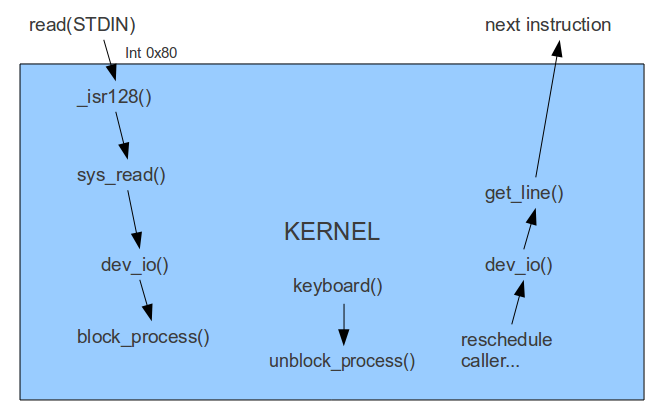
\includegraphics[scale=0.5]{../img/syscall.png}
\end{center}


- El proceso ejecuta "read(STDIN\_FILENO, buf, len)", que consiste en poner los
valores correspondientes en ebx, ecx y edx, poner el número de la system call
en eax, y realizar un "int 0x80". Más sobre esto en la sección "Utilidades".

- Se atiende la interrupción en kernel/isr.asm, en la etiqueda \_isr128 (128
= 0x80). Esta función se encarga de guardar el valor de los registros, armar
la pila con los parametros y llamar a la rutina de atención correspondiente
al número ingresado en eax.

- En este caso caemos en sys\_read(), que se encuentra en fs/fs.c. Esta función
recobra el inodo correspondiente al descriptor de archivo ingresado
(STDIN\_FILENO = 0, que es un fd inicializado cuando se creo el proceso,
apuntando al inodo /dev/stdin). Se pregunta si el inodo corresponde a un
dispositivo de caracteres, que resulta ser verdadero en este caso, y en
consecuencia llama a dev\_io(), la función que hace I/O de dispositivos.

- dev\_io() se encuentra en kernel/dev.c. Actualmente esta función solo atiende
peticiones para STDIN, STDOUT ó STDERR (aunque debería ser genérica y atender
cualquier dispositivo de entrada/salida). En este caso el dispositivo es STDIN,
y como se pide leer del mismo, se llama a la función block\_process().

- block\_process() se encuentra en kernel/sched.c, proceso se bloquea en este
punto, esperando la respuesta del dispositivo en cuestion (el teclado). Esto
simplemente significa remover al processo de la lista ready, agregarlo a la
lista wait, y llamar a schedule() para dar lugar a otro proceso. En nuestro
sistema esto probablemente significa que pasamos al estado idle.

- El proceso se mantiene bloqueado, hasta que por el teclado es enviada la
tecla '\textbackslash n' (el enter). Esta es nuestra señal para enviar los
datos al proceso que los pidio. Por ende la función keyboard() (que es la
que recibió la interrupcion con el '\textbackslash n' del teclado) llama a
unblock\_process(), que desbloquea al primer proceso que estuviese esperando
un dispositivo, en este caso el teclado.

- unblock\_process() tambien se encuentra en kernel/sched.c, busca en la lista
de procesos bloqueados el primero correspondiente al dispositivo en cuestion,
y lo agrega nuevamente a la lista ready. Luego sigue la ejecución del proceso
que fue interrumpido por el teclado.

- Llega el momento en que el scheduler programa nuevamente al proceso que
inició la llamada read(). Este vuelve al punto en donde se bloqueo, es decir en
dev\_io(). La siguiente linea luego de la llamada block\_process() es una
llamada a get\_line(), que esta garantizada que funcionará ya que fuimos
despertados por el teclado por esta razón. Luego se llena el buffer con lo
recibido por la consola, se recobra el estado de los registros y se realiza el
anticipado iret de \_isr128().

Esto concluye la atención a esta llamada al sistema.

Resumiendo, el kernel realiza en el booteo la inicialización de los siguiente
componentes en orden (ver kernel/kernel.asm): A20, GDT, IDT, Modo Protegido,
System calls, MMU, Paginación, Clock, File System, Scheduler y habilita
interrupciones. Antes de habilitar interrupciones se agrega a la lista ready un
proceso "cash" (crappy *** shell), la shell que termina manejando el hilo de
ejecución. Luego el sistema esta en manos del usuario.
